\chapter{La tabla periódica: un primer vistazo}\label{ch:g9:periodic-table-first-look}

En la pared de casi todas las aulas de química cuelga el mismo cuadro:
118 casillas, cada una con un símbolo y un número, ordenadas en filas y
columnas con una forma extraña: torres altas a los lados, un hueco en
el centro y dos filas sueltas debajo. Cuando se dibujó por primera vez,
en 1869, tenía unas sesenta casillas y varias vacías. Su autor se atrevió
a describir los elementos que algún día llenarían los huecos, y acertó.

\begin{recall}
Un \omterm{def:g9:inside-the-atom:element}{elemento químico} es el conjunto de los \omterm{def:g7:atoms-and-molecules:atom}{átomos} con el mismo \omterm{def:g9:inside-the-atom:atomic-number}{número
atómico} $Z$, el número de \omterm{def:g9:inside-the-atom:proton}{protones} del \omterm{def:g9:inside-the-atom:nucleus}{núcleo} (\cref{ch:g9:inside-the-atom}).
Cada elemento tiene un símbolo, una letra mayúscula a veces seguida de
una minúscula (\cref{ch:g7:atoms-and-molecules}). Los \omterm{def:g9:periodic-table-first-look:metal}{metales} como el
hierro, el cinc y el aluminio dan \omterm{def:g9:ions:ion}{iones} positivos (\cref{ch:g9:ions}).
\end{recall}

\section{Una tabla de los elementos}

\begin{definition}[Tabla periódica]\label{def:g9:periodic-table-first-look:periodic-table}
La \emph{tabla periódica}\index{tabla periodica@tabla periódica} enumera todos los
\omterm{def:g9:inside-the-atom:element}{elementos químicos} por orden creciente de \omterm{def:g9:inside-the-atom:atomic-number}{número atómico}, de $Z = 1$ a
$Z = 118$, dispuestos en filas de modo que los elementos de propiedades
parecidas quedan en la misma columna.
\end{definition}

\begin{definition}[Periodo y grupo]\label{def:g9:periodic-table-first-look:period}
Una fila de la \omterm{def:g9:periodic-table-first-look:periodic-table}{tabla periódica} es un \emph{periodo}\index{periodo}; hay
siete. Una columna es un \emph{grupo}\index{grupo}; hay dieciocho,
numerados del 1 al 18 de izquierda a derecha. Las dos filas impresas
debajo de la tabla pertenecen a los periodos 6 y 7; se colocan aparte
solo para que la tabla no sea demasiado ancha.
\end{definition}

\begin{omfigure}
\omperiodictable[colour=metals, legend=true, cell=0.86cm]

{\small La \omterm{def:g9:periodic-table-first-look:periodic-table}{tabla periódica}. Cada casilla da el \omterm{def:g9:inside-the-atom:atomic-number}{número atómico} y el
símbolo. Colores: \omterm{def:g9:periodic-table-first-look:metal}{metales}, metaloides (elementos intermedios entre los
\omterm{def:g9:periodic-table-first-look:metal}{metales} y los \omterm{def:g9:periodic-table-first-look:metal}{no metales}) y \omterm{def:g9:periodic-table-first-look:metal}{no metales}, según la clasificación habitual.}
\end{omfigure}

\begin{method}[Leer la tabla periódica]\label{met:g9:periodic-table-first-look:read}
Para situar un elemento:
\begin{enumerate}
  \item se busca su casilla a partir de su símbolo o de su \omterm{def:g9:inside-the-atom:atomic-number}{número
        atómico};
  \item su fila da su \omterm{def:g9:periodic-table-first-look:period}{periodo}, y su columna, su grupo;
  \item su color indica si es un \omterm{def:g9:periodic-table-first-look:metal}{metal} o un \omterm{def:g9:periodic-table-first-look:metal}{no metal}.
\end{enumerate}
El sodio, \ce{Na}, $Z = 11$: \omterm{def:g9:periodic-table-first-look:period}{periodo} 3, \omterm{def:g9:periodic-table-first-look:period}{grupo} 1, un \omterm{def:g9:periodic-table-first-look:metal}{metal}. El cloro,
\ce{Cl}, $Z = 17$: \omterm{def:g9:periodic-table-first-look:period}{periodo} 3, \omterm{def:g9:periodic-table-first-look:period}{grupo} 17, un \omterm{def:g9:periodic-table-first-look:metal}{no metal}.
\end{method}

\section{Metales y no metales}

\begin{definition}[Metal y no metal]\label{def:g9:periodic-table-first-look:metal}
Un \emph{metal}\index{metal} es un elemento que, como \omterm{def:g6:pure-substances-and-mixtures:pure-substance}{sustancia pura},
brilla cuando está recién cortado, conduce bien la electricidad y el
calor, se puede doblar o moldear a martillazos, y forma \omterm{def:g9:ions:ion}{iones}
positivos. Un \emph{no metal}\index{no metal} carece de estas
propiedades: muchos son gases (el oxígeno, el nitrógeno, el cloro), los
que son sólidos son mates y quebradizos (el azufre, el carbono en forma
de carbón), y tienden a formar \omterm{def:g9:ions:ion}{iones} negativos o a compartir \omterm{def:g9:inside-the-atom:nucleus}{electrones}
en \omterm{def:g7:atoms-and-molecules:molecule}{moléculas}.
\end{definition}

\begin{proposition}[Dónde se sitúan]\label{prop:g9:periodic-table-first-look:where}
Alrededor de cuatro de cada cinco elementos son \omterm{def:g9:periodic-table-first-look:metal}{metales}; ocupan la
izquierda y el centro de la tabla. Los \omterm{def:g9:periodic-table-first-look:metal}{no metales} están arriba a la
derecha, con el hidrógeno solo arriba a la izquierda. A lo largo de la
frontera entre unos y otros, unos pocos elementos (el boro, el silicio,
el germanio, el arsénico, el antimonio y el teluro) tienen propiedades
intermedias: son los metaloides.
\end{proposition}

\section{Columnas que se comportan igual}

\begin{proposition}[Los elementos de un grupo se comportan igual]\label{prop:g9:periodic-table-first-look:alike}
Los elementos de un mismo grupo reaccionan de maneras parecidas y forman
compuestos parecidos. El litio, el sodio y el potasio, arriba del \omterm{def:g9:periodic-table-first-look:period}{grupo}
1, son \omterm{def:g9:periodic-table-first-look:metal}{metales} blandos que reaccionan con el agua desprendiendo
hidrógeno; la reacción es más violenta cuanto más abajo en el grupo. El
flúor, el cloro, el bromo y el yodo, del \omterm{def:g9:periodic-table-first-look:period}{grupo} 17, son \omterm{def:g9:periodic-table-first-look:metal}{no metales} de
color que reaccionan con los \omterm{def:g9:periodic-table-first-look:metal}{metales} formando sales. El helio, el neón,
el argón y los demás elementos del \omterm{def:g9:periodic-table-first-look:period}{grupo} 18 casi no reaccionan con nada.
\end{proposition}

\begin{inthelab}[Litio, sodio y potasio en agua]
Detrás de una pantalla de protección, el profesor echa un trocito de
litio del tamaño de un grano de arroz en un barreño grande de agua:
burbujea suavemente. Un trozo de sodio del mismo tamaño corre por la
superficie, fundiéndose en una bolita plateada. El potasio \omterm{def:g4:what-a-fire-needs:burning}{arde} enseguida
con una llama lila. Los tres desprenden hidrógeno y dejan una \omterm{def:g9:acids-bases-ph:acidic}{disolución
básica}.
\end{inthelab}

\begin{safety}{\ghs[0.82cm]{GHS02}\ghs[0.82cm]{GHS05}}
% ledger: ghs:Na
Sodio: en contacto con el agua desprende gases inflamables que pueden
inflamarse espontáneamente (GHS02); provoca quemaduras graves (GHS05). Se
guarda bajo aceite y solo lo manipula el profesor, con pinzas y en
trozos diminutos.
\end{safety}

\section{La idea de Mendeléiev}

\begin{history}[Los huecos de Mendeléiev, 1869--1886]
En 1869, Dmitri Mendeléiev ordenó los elementos conocidos entonces por
orden creciente de peso atómico (la masa de sus \omterm{def:g7:atoms-and-molecules:atom}{átomos} comparada con la
del hidrógeno) y colocó juntos los que tenían propiedades parecidas.
Donde el patrón lo exigía, dejó huecos para elementos que nadie había
encontrado aún, y en 1871 describió sus propiedades: debajo del silicio,
un ``eka-silicio'' cuyo peso atómico sería de alrededor de 72. En 1886,
el químico Clemens Winkler descubrió el germanio en un mineral de plata,
midió su peso atómico, 72.3, y vio que era el elemento que faltaba. El
galio (1875) y el escandio (1879) llenaron también huecos que había
dejado Mendeléiev.
\end{history}

\begin{omfigure}
\begin{minipage}[b]{0.32\linewidth}\centering
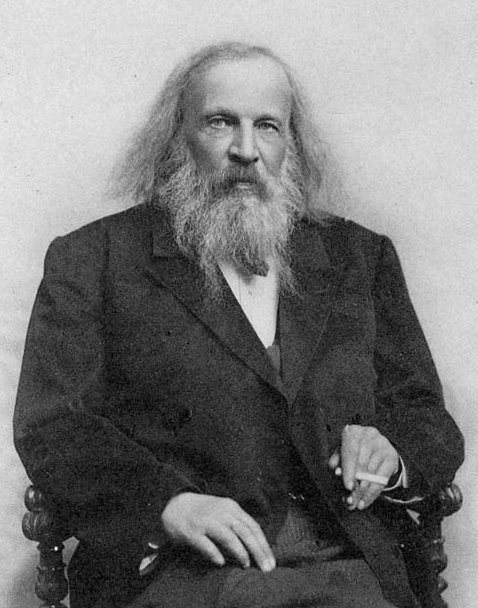
\includegraphics[width=\linewidth]{images/book1/mendeleev.jpg}

{\small Dmitri Mendeléiev (1834--1907).}
\end{minipage}\hfill
\begin{minipage}[b]{0.6\linewidth}\centering
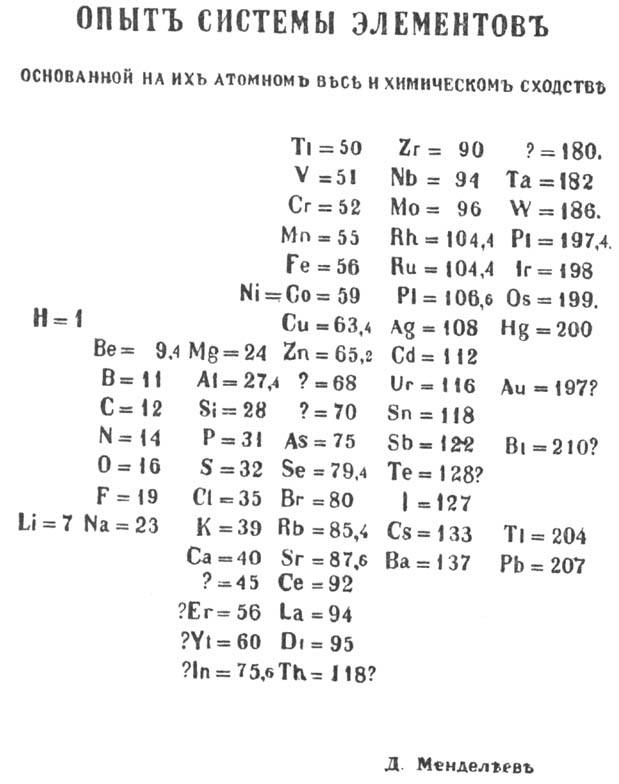
\includegraphics[width=0.85\linewidth]{images/book1/mendeleev-1869.jpg}

{\small La tabla de Mendeléiev de 1869, en ruso. Junto a Si $= 28$ y
Al $= 27.4$, los huecos ``? $= 70$'' y ``? $= 68$'' esperan al germanio
y al galio.}
\end{minipage}
\end{omfigure}

\begin{remark}[Ordenar por número atómico]\label{rem:g9:periodic-table-first-look:order}
Mendeléiev ordenó los elementos por peso atómico, y tuvo que
intercambiar algunas parejas, como el teluro y el yodo, para mantener
juntas las familias. Hoy la tabla se ordena por \omterm{def:g9:inside-the-atom:atomic-number}{número atómico},
descubierto más tarde, y esos intercambios ya no hacen falta.
\end{remark}

\section{Ejercicios}

\begin{exercise}[$\star$]\label{exo:g9:periodic-table-first-look:1}
¿En qué orden se colocan los elementos en la \omterm{def:g9:periodic-table-first-look:periodic-table}{tabla periódica}?
\end{exercise}

\begin{exercise}[$\star$]\label{exo:g9:periodic-table-first-look:2}
Da el \omterm{def:g9:periodic-table-first-look:period}{periodo} y el grupo del carbono ($Z = 6$), el magnesio ($Z = 12$)
y el argón ($Z = 18$).
\end{exercise}

\begin{exercise}[$\star$]\label{exo:g9:periodic-table-first-look:3}
¿\omterm{def:g9:periodic-table-first-look:metal}{Metal} o \omterm{def:g9:periodic-table-first-look:metal}{no metal}: el hierro, el azufre, el cobre, el oxígeno, el
aluminio, el cloro?
\end{exercise}

\begin{exercise}[$\star$]\label{exo:g9:periodic-table-first-look:4}
¿Qué elemento está justo debajo del sodio en la tabla? ¿Y justo debajo
del cloro?
\end{exercise}

\begin{exercise}[$\star\star$]\label{exo:g9:periodic-table-first-look:5}
Con la tabla, nombra el elemento del \omterm{def:g9:periodic-table-first-look:period}{periodo} 4 y \omterm{def:g9:periodic-table-first-look:period}{grupo} 2, y el elemento
del \omterm{def:g9:periodic-table-first-look:period}{periodo} 2 y \omterm{def:g9:periodic-table-first-look:period}{grupo} 15.
\end{exercise}

\begin{exercise}[$\star\star$]\label{exo:g9:periodic-table-first-look:6}
¿Por qué cabe esperar que el potasio reaccione con el agua, como el
sodio?
\end{exercise}

\begin{exercise}[$\star\star$]\label{exo:g9:periodic-table-first-look:7}
Un elemento brillante conduce la electricidad y forma el \omterm{def:g9:ions:ion}{ion}
\ce{X^{2+}}. ¿Es un \omterm{def:g9:periodic-table-first-look:metal}{metal} o un \omterm{def:g9:periodic-table-first-look:metal}{no metal}? Explícalo.
\end{exercise}

\begin{exercise}[$\star\star$]\label{exo:g9:periodic-table-first-look:8}
¿Por qué dejó Mendeléiev huecos en su tabla? ¿Por qué era esto un punto
fuerte de su tabla y no una debilidad?
\end{exercise}

\begin{exercise}[$\star\star$]\label{exo:g9:periodic-table-first-look:9}
Mira la tabla de Mendeléiev de 1869. ¿Qué pesos atómicos daba para el
carbono y para el oxígeno? ¿Qué dos huecos, marcados con un signo de
interrogación, aparecen junto al aluminio y al silicio?
\end{exercise}

\begin{exercise}[$\star\star$]\label{exo:g9:periodic-table-first-look:10}
¿Cuántos elementos hay en el \omterm{def:g9:periodic-table-first-look:period}{periodo} 2? ¿Y en el \omterm{def:g9:periodic-table-first-look:period}{periodo} 4?
\end{exercise}

\begin{exercise}[$\star\star\star$]\label{exo:g9:periodic-table-first-look:11}
El helio, el neón y el argón casi no reaccionan con nada. ¿En qué grupo
están? ¿Para qué podrían usarse, dada esta propiedad?
\end{exercise}

\begin{exercise}[$\star\star\star$]\label{exo:g9:periodic-table-first-look:12}
El galio, debajo del aluminio, se descubrió en 1875. Mendeléiev le
había predicho un peso atómico cercano a la media de sus vecinos, el
aluminio (27.0) y el indio (114.8). Calcula esa media. (Galio: 69.7.)
\end{exercise}

\section{Problema: El hueco de Mendeléiev}

\begin{problem}[{Problema de fin de semana --- predecir el peso atómico
de un elemento que falta a partir de sus cuatro vecinos}]
\label{pb:g9:periodic-table-first-look:1}
% ledger: aw:Si, aw:Sn, aw:Ga, aw:As, aw:Ge, mend:eka-si-aw, ge:winkler-aw
En 1871, Mendeléiev predijo las propiedades del eka-silicio, el
elemento que faltaba debajo del silicio. Una de sus ideas era que las
propiedades de un elemento se sitúan entre las de sus vecinos de arriba
y de abajo, de la izquierda y de la derecha. Los pesos atómicos actuales
de los cuatro vecinos del hueco son: silicio 28.1 (arriba), estaño 118.7
(abajo), galio 69.7 (izquierda), arsénico 74.9 (derecha).

\medskip
\noindent\textbf{Parte I --- El hueco.}
\begin{enumerate}
  \item Con la \omterm{def:g9:periodic-table-first-look:periodic-table}{tabla periódica} de este capítulo, halla el \omterm{def:g9:inside-the-atom:atomic-number}{número
        atómico}, el \omterm{def:g9:periodic-table-first-look:period}{periodo} y el grupo del germanio, el elemento que
        llena el hueco.
  \item ¿Qué elemento está encima de él, cuál debajo, cuál a su
        izquierda y cuál a su derecha?
  \item ¿El germanio es un \omterm{def:g9:periodic-table-first-look:metal}{metal}, un \omterm{def:g9:periodic-table-first-look:metal}{no metal} o un metaloide?
  \item ¿Por qué esperaba Mendeléiev que el elemento que faltaba se
        pareciera al silicio?
\end{enumerate}

\medskip
\noindent\textbf{Parte II --- Medias.}
\begin{enumerate}[resume]
  \item Calcula la media de los pesos atómicos de los elementos de
        encima y de debajo del hueco.
  \item Calcula la media de los pesos atómicos de los elementos de la
        izquierda y de la derecha.
  \item ¿Cuál de las dos medias se acerca más al peso atómico real del
        germanio, 72.6? ¿A qué podría deberse?
  \item En su tabla de 1869, Mendeléiev había escrito ``? $= 70$'' para
        este hueco. ¿Por cuánto se equivocó?
\end{enumerate}

\medskip
\noindent\textbf{Parte III --- La predicción.}
\begin{enumerate}[resume]
  \item Calcula la media de los cuatro vecinos, con un decimal.
  \item En 1871, Mendeléiev predijo 72; en 1886, Winkler midió 72.3.
        Compáralo con tu media.
  \item ¿Por qué el descubrimiento del germanio convenció a muchos
        químicos de que la tabla de Mendeléiev era correcta?
  \item Enuncia tu predicción: el peso atómico del eka-silicio a partir
        de la media de sus cuatro vecinos.
\end{enumerate}
\end{problem}
